\documentclass[11pt,a4paper]{scrartcl}
\usepackage[top=3cm,bottom=3cm,left=2cm,right=2cm]{geometry} % Seitenränder einstellen
\usepackage[utf8]{inputenc} % Umlaute im Text
\usepackage[english]{babel} % Worttrennung nach der neuen Rechtschreibung und deutsche Bezeichnungen
\usepackage[dvipsnames]{xcolor} % Farbe in Dokument
\parindent 0pt % kein Einrücken bei neuem Absatz
\usepackage{amsmath} % zusätzliche mathematische Umgebungen
\usepackage{amssymb} % zusätzliche mathematische Symbole
%\usepackage{bbold} % zusätzliche mathematische Symbole
\usepackage{units} % schöne Einheiten und Brüche
\usepackage{icomma} % kein Leerzeichen bei 1,23 in Mathe-Umgebung
\usepackage{wrapfig} % von Schrift umflossene Bilder und Tabellen
\usepackage{picinpar} % Objekt in Fließtext platzieren (ähnlich zu wrapfig)
\usepackage{scrhack} % verbessert andere Pakete, bessere Interaktion mit KOMA-Skript
\usepackage{float} % bessere Anpassung von Fließobjekten
\usepackage{pgf} % Makro zur Erstellung von Graphiken
\usepackage{tikz} % Benutzeroberfläche für pgf
\usepackage[margin=10pt,font=small,labelfont=bf,labelsep=endash,format=plain]{caption} % Einstellungen für Tabellen und Bildunterschriften

\usepackage{graphicx}
\graphicspath{ {U5_Ex5/} }

\usepackage{listings}
\usepackage{subcaption} % Unterschriften für mehrere Bilder
\usepackage{enumitem} % no indentation at description environment
\usepackage[onehalfspacing]{setspace} % Änderung des Zeilenabstandes (hier: 1,5-fach)
\usepackage{booktabs} % Einstellungen für schönere Tabellen
\usepackage{graphicx} % Einfügen von Grafiken -> wird in master-file geladen
\usepackage{url} % URL's (z.B. in Literatur) schöner formatieren
\usepackage[pdftex]{hyperref} % Verweise innerhalb und nach außerhalb des PDF; hyperref immer als letztes Paket einbinden

% define bordermatrix with brackets

\makeatletter
\def\bbordermatrix#1{\begingroup \m@th
  \@tempdima 4.75\p@
  \setbox\z@\vbox{%
    \def\cr{\crcr\noalign{\kern2\p@\global\let\cr\endline}}%
    \ialign{$##$\hfil\kern2\p@\kern\@tempdima&\thinspace\hfil$##$\hfil
      &&\quad\hfil$##$\hfil\crcr
      \omit\strut\hfil\crcr\noalign{\kern-\baselineskip}%
      #1\crcr\omit\strut\cr}}%
  \setbox\tw@\vbox{\unvcopy\z@\global\setbox\@ne\lastbox}%
  \setbox\tw@\hbox{\unhbox\@ne\unskip\global\setbox\@ne\lastbox}%
  \setbox\tw@\hbox{$\kern\wd\@ne\kern-\@tempdima\left[\kern-\wd\@ne
    \global\setbox\@ne\vbox{\box\@ne\kern2\p@}%
    \vcenter{\kern-\ht\@ne\unvbox\z@\kern-\baselineskip}\,\right]$}%
  \null\;\vbox{\kern\ht\@ne\box\tw@}\endgroup}
\makeatother

% make Titel
\title{Mining massive Datasets WS 2017/18}
\subtitle{Problem Set 7}
\author{Rudolf Chrispens, Marvin Klaus, Daniela Schacherer}

\begin{document}

\maketitle

\section*{Exercise 01}

\begin{itemize}
	\item Internally an array is used to store both - key and value - as an object of the so-called Entry class. For handling collisions meaning values that map to the same key a linked list is further used. 
	\item A new key-value pair is added by the put-method. This method calculates the hash value for a given key and uses it as index in the hash table. If the calculated index position already holds a key-value pair, the linked list at this position is used and the key-value pair is stored at the first available position in this list. The function is also responsible for resizing the table if appropriate.
	\item When one wants to search given a key the corresponding index is calculated. At the calculated position the key is compared to the given search key and if it matches the corresponding value is returned. If it doesn't match, each entry of the linked list at this hash map position is searched through until the matching key is found. If the key does not exist this is also returned to the user.
\end{itemize} 

\section*{Exercise 02}

\section*{Exercise 03}

If I understand that Question right I just should plot and look at whcih point the lines exceeds the value 0.5? If so then here the approximate values for each plot. I write the values for each $r$ in a list that show the value of $b$ as [10, 20, 50, 100].

\begin{itemize}
    \item [r=2] - [0.26, 0.18, 0.13, -] (Figure \ref{fig:r2})
    \item [r=3] - [0.4, 0.32, 0.23, 0.18] (Figure \ref{fig:r3})
    \item [r=5] - [0.58, 0.5, 0.42, 0.34] (Figure \ref{fig:r5})
    \item [r=7] - [0.67, 0.62, 0.53, 0.48] (Figure \ref{fig:r7})
\end{itemize}

\begin{figure}
\centering
\begin{minipage}{.5\textwidth}
  \centering
  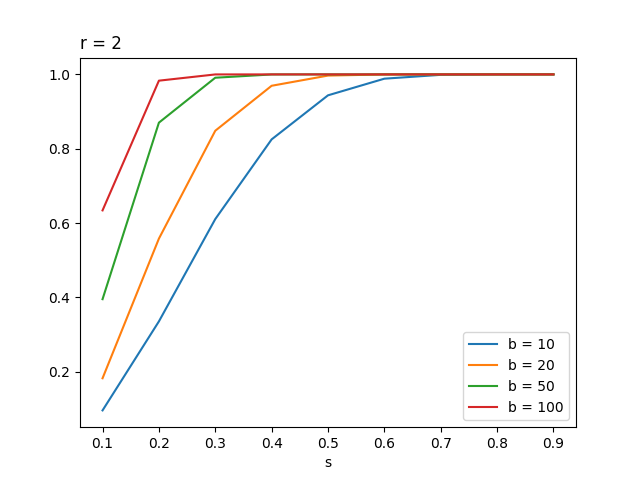
\includegraphics[width=.99\linewidth]{q3r2}
  \captionof{figure}{r = 2}
  \label{fig:r2}
\end{minipage}%
\begin{minipage}{.5\textwidth}
  \centering
  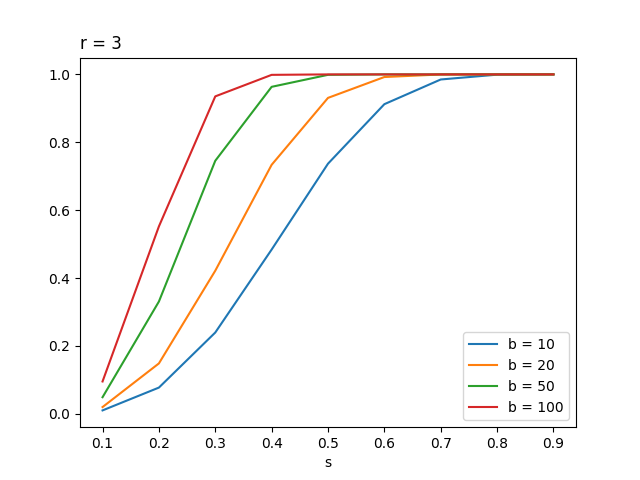
\includegraphics[width=.99\linewidth]{q3r3}
  \captionof{figure}{r = 3}
  \label{fig:r3}
\end{minipage}
\end{figure}

\begin{figure}
\centering
\begin{minipage}{.5\textwidth}
  \centering
  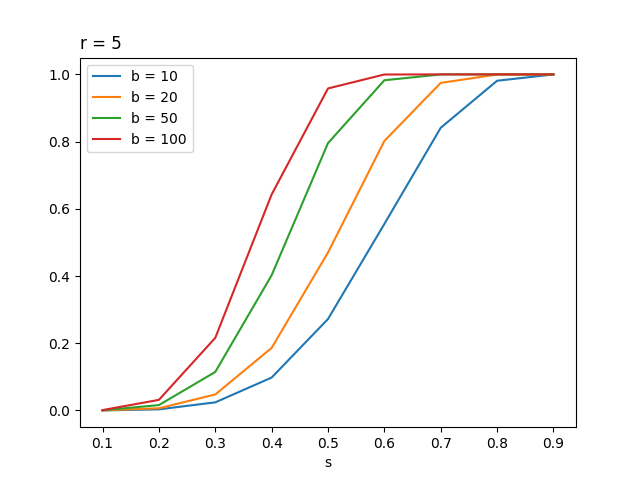
\includegraphics[width=.99\linewidth]{q3r5}
  \captionof{figure}{r = 5}
  \label{fig:r5}
\end{minipage}%
\begin{minipage}{.5\textwidth}
  \centering
  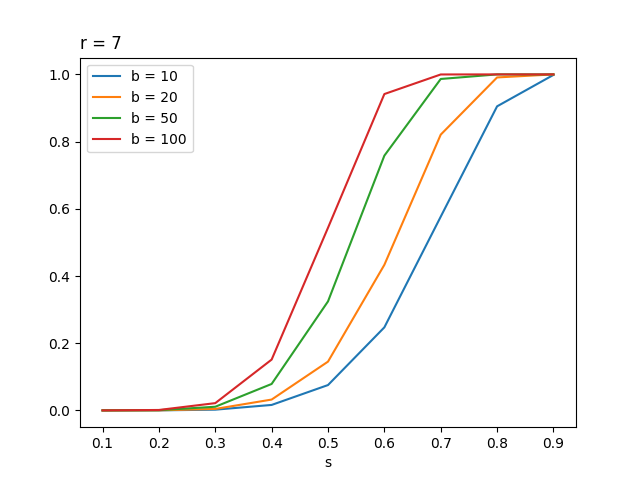
\includegraphics[width=.99\linewidth]{q3r7}
  \captionof{figure}{r = 7}
  \label{fig:r7}
\end{minipage}
\end{figure}

\section*{Exercise 04}

\end{document}
